\documentclass[twocolumn,9pt]{article}

\usepackage[margin=0.8in,bottom=1.25in,columnsep=.4in]{geometry}
\usepackage{amsmath}
\usepackage{amssymb}
\usepackage{listings}
\usepackage{color}
\usepackage{cite}
\usepackage{graphicx}
\usepackage{multicol}
 
\definecolor{codegreen}{rgb}{0,0.6,0}
\definecolor{codegray}{rgb}{0.5,0.5,0.5}
\definecolor{codepurple}{rgb}{0.58,0,0.82}
 
\lstdefinestyle{code}{
	% backgroundcolor=\color{bggray},
  commentstyle=\color{codegray},
  keywordstyle=\color{codegreen}\bfseries,
  stringstyle=\color{codepurple},
  basicstyle=\ttfamily\footnotesize,
  breakatwhitespace=false,     
  breaklines=true,         
  captionpos=b,          
  keepspaces=true,                  
  showspaces=false,        
  showstringspaces=false,
  showtabs=false,          
  tabsize=2
}
 
\lstset{style=code}

\title{
	50.039 Theory and Practice of Deep Learning\\
	Coding Homework 5
}

\author{Joel Huang 1002530}
\date{\today}

\begin{document}
\maketitle
\section{Custom dataset class}
We write a custom dataset class with the ability to load image and label paths,
and implement a static method \lstinline{train_val_test_split()} to automatically
split the dataset into the training, validation, and test sets.

\subsection*{Constructor}
The class constructor takes the directory path containing the images, a file containing
all the image paths, a \lstinline{.npy} file containing all the labels, and loads a Pandas
\lstinline{DataFrame} with keys as image paths and values as their corresponding labels. 
\begin{lstlisting}[language=Python]
class FlowerDataset(Dataset):
  def __init__(self, image_dir, image_paths, label_file, transform=None):
    self.image_dir = image_dir
    self.labels = np.load(label_file)
    self.image_label_pairs = self._load_paths(image_paths)
    self.transform = transform
\end{lstlisting}

\subsection*{Subclass implementations}
We need to necessarily implement \lstinline{__len__()} and \lstinline{__getitem__()} since
we are subclassing \lstinline{torch.utils.data.Dataset}. To be more efficient, we only load
images when the item is accessed via \lstinline{dataset[index]}.
\begin{lstlisting}[language=Python]
  def __len__(self):
    return len(self.image_label_pairs)
  
  def __getitem__(self, idx):
    # apply transforms
    image_path = self.image_label_pairs.index[idx]
    image = self._load_image(image_path)
    if self.transform is not None:
      image = self.transform(image)
    label = self.labels[idx]
    return {'image': image,
        'label': label}
\end{lstlisting}

\subsection*{Loading data}
Two private methods here for data loading. The first method \lstinline{_load_paths()} constructs
a Pandas \lstinline{DataFrame} object containing the image paths and their corresponding labels.
The second method \lstinline{_load_image()} loads an image from the given path as a \lstinline{PIL.Image}.
Single-channel (grayscale) images are stacked into 3-channel images here using \lstinline{numpy.repeat()}.
\begin{lstlisting}[language=Python]   
  def _load_paths(self, file_path):
    """
    params:  file_path, a path pointing to where the image paths are stored.
    returns: dictionary with keys 'full_image_path', and values 'label'
    """
    split_set = {}
    with open(file_path) as f:
      lines = f.readlines()
      num_lines = len(lines)
      assert(num_lines == len(self.labels))
      for line_num in range(num_lines):
        full_image_path = os.path.join(self.image_dir, lines[line_num].strip('\n'))
        split_set[full_image_path] = self.labels[line_num]
    return pd.DataFrame.from_dict(split_set, orient='index')

  def _load_image(self, image_path):
    img = Image.open(image_path)
    img.load()
    img = np.array(img)
    if len(img.shape) == 2:
      img = np.expand_dims(img, 2)
      img = np.repeat(img, 3, 2)
    return Image.fromarray(img)
\end{lstlisting}

\subsection*{Implementing splits}
In the final class method, we implement a method to split the dataset into
training, validation and test sets. This returns three splits with type
\lstinline{torch.utils.data.Subset}, which can be directly fed into the
\lstinline{torch.utils.data.DataLoader} class.
\begin{lstlisting}[language=Python]
  def train_val_test_split(self, train_ratio, val_ratio):
    dataset_length = len(self.image_label_pairs)
    train_length = int(train_ratio * dataset_length)
    val_length = int(val_ratio * dataset_length)
    test_length = len(self) - train_length - val_length
    splits = [train_length, val_length, test_length]
    return random_split(self, splits)
\end{lstlisting}

\section{Data loading}
\subsection*{Data augmentation and split ratio}
We apply only a center crop of size $200$. A training, validation, test split of
$0.7, 0.1, 0.2$ is carried out using our split function above:
\begin{lstlisting}[language=Python]
transform = transforms.Compose([transforms.CenterCrop(200), transforms.ToTensor()])
dataset = FlowerDataset('data', 'image_paths.txt', 'labels.npy', transform=transform)
train_set, val_set, test_set = dataset.train_val_test_split(0.7, 0.1)
\end{lstlisting}

\subsection*{Batch size}
We then construct three loaders for each of the sets with a \lstinline{batch_size} of 32.
\begin{lstlisting}[language=Python]
train_loader = DataLoader(train_set, batch_size=32, shuffle=True, num_workers=4)
val_loader = DataLoader(val_set, batch_size=32, shuffle=True, num_workers=4)
test_loader = DataLoader(test_set, batch_size=32, shuffle=True, num_workers=4)
\end{lstlisting}

\section{Loss function}
We choose \lstinline{CrossEntropyLoss} for our $102$-class dataset. Categorical cross entropy
loss is the natural choice for multi-class classification.

\section{Hyperparameters and optimizer}
After validating over a small number of epochs, we choose a learning rate of $10^{-3}$ and a
batch size of $32$. We use SGD with momentum.
\begin{lstlisting}[language=Python]
batch_size = 32
num_epochs = 50
learning_rate = 1e-3

optimizer = optim.SGD(model.parameters(), lr=learning_rate, momentum=0.9)
CE = nn.CrossEntropyLoss()
\end{lstlisting}

\section{Task I: Training all layers of ResNet18}
\subsection*{Initializing the model}
We can initialize an untrained model with a custom number of classes using the \lstinline{num_classes}
argument. Examining the PyTorch source code, this passes the number of classes into the \lstinline{ResNet}
constructor, which builds a FC layer with that number of classes.
\begin{lstlisting}[language=Python]
model = models.resnet18(num_classes=102).to(device)
\end{lstlisting}

\subsection*{Training and validation results}
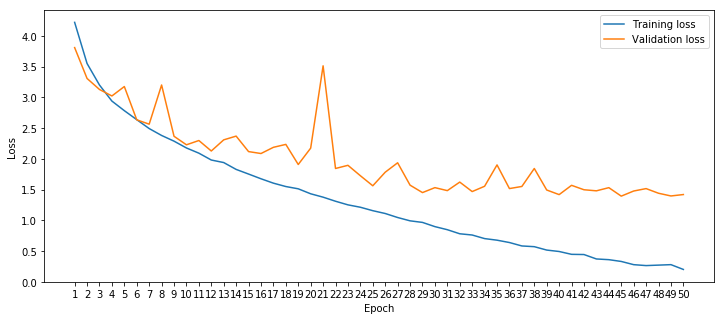
\includegraphics[width=\columnwidth]{task1.png}
We observe the training loss decreasing and the validation loss decreasing but not converging. The best
epoch's results:
\begin{lstlisting}
Epoch: 45
Training set: Average loss: 0.3338
Validation set: Average loss: 1.3952, Accuracy: 540/818 (66%)
Saving model (epoch 45) with lowest validation loss: 1.395247207238124
\end{lstlisting}

\subsection*{Test accuracy: 62$\%$}
This model (epoch 45) fairs decently on the test set:
\begin{lstlisting}
Test set: Accuracy: 1011/1639 (62%)
\end{lstlisting}

\section{Task II: Training over pretrained ResNet18}
\subsection*{Initializing the model}
We can initialize an pretrained model with a custom number of classes using the \lstinline{pretrained=True}
argument. However, we cannot specify the number of classes using the same method in Task I. Instead, we have
to explicitly reset the FC layer:
\begin{lstlisting}[language=Python]
model = models.resnet18(pretrained=True)
model.fc = nn.Linear(512, 102)
model.to(device)
\end{lstlisting}

\subsection*{Training and validation results}
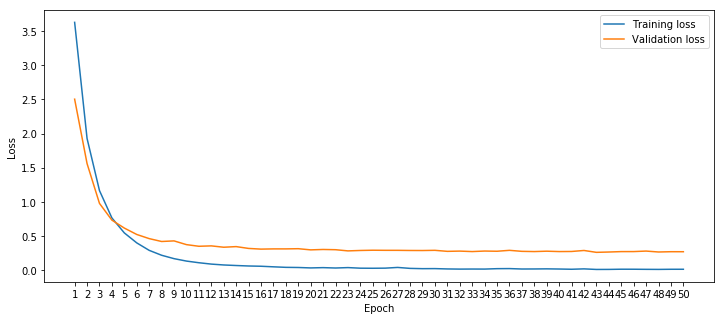
\includegraphics[width=\columnwidth]{task2.png}
We observe the both training loss and the validation loss decreasing and converging. The best
epoch's results:
\begin{lstlisting}
Epoch: 43
Training set: Average loss: 0.0107
Validation set: Average loss: 0.2609, Accuracy: 770/818 (94%)
Saving model (epoch 43) with lowest validation loss: 0.26094281100309813
\end{lstlisting}

\subsection*{Test accuracy: 93$\%$}
This model (epoch 43) fairs well on the test set:
\begin{lstlisting}
Test set: Accuracy: 1522/1639 (93%)
\end{lstlisting}

\section{Task III: Training 2 pre-final layers of ResNet18}
\subsection*{Initializing the model}
In ResNet18, the forward pass is:
\begin{lstlisting}[language=Python]
def forward(self, x):
  x = self.conv1(x)
  x = self.bn1(x)
  x = self.relu(x)
  x = self.maxpool(x)

  x = self.layer1(x)
  x = self.layer2(x)
  x = self.layer3(x)
  x = self.layer4(x)

  x = self.avgpool(x)
  x = x.view(x.size(0), -1)
  x = self.fc(x)
\end{lstlisting}

We can train only the 2 pre-final layers (\lstinline{layer3, layer4}) by loading the pre-trained model, then setting the \lstinline{requires_grad} attribute of the parameters outside these two layers to \lstinline{False}. The \lstinline{relu}, \lstinline{maxpool}, and \lstinline{avgpool} layers do not contain any parameters, so they are not frozen. We write a function \lstinline{freeze()} to freeze the gradient in the parameters in the layer.

\begin{lstlisting}[language=Python]
def freeze(layer):
    for param in layer.parameters():
        param.requires_grad = False

model = models.resnet18(pretrained=True)

# freeze all layers before layer3
freeze(model.conv1)
freeze(model.bn1)
freeze(model.layer1)
freeze(model.layer2)
model.fc = nn.Linear(512, 102)

model.to(device)
\end{lstlisting}

\subsection*{Training and validation results}
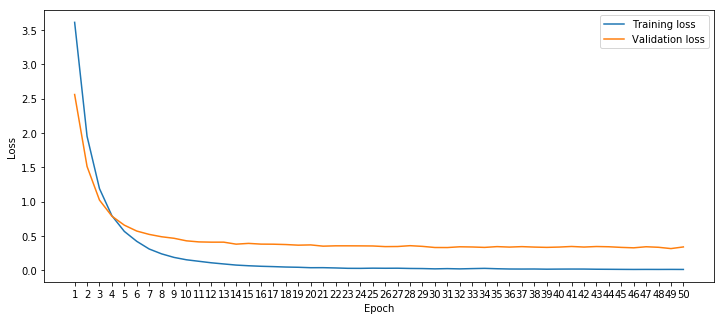
\includegraphics[width=\columnwidth]{task3.png}
We observe the both training loss and the validation loss decreasing and converging. The best
epoch's results:
\begin{lstlisting}
Epoch: 49
Training set: Average loss: 0.0114
Validation set: Average loss: 0.3148, Accuracy: 756/818 (92%)
Saving model (epoch 49) with lowest validation loss: 0.31477418828469056
\end{lstlisting}

\subsection*{Test accuracy: 92$\%$}
This model (epoch 49) fairs well on the test set:
\begin{lstlisting}
Test set: Accuracy: 1503/1639 (92%)
\end{lstlisting}
\end{document}